%% ─────────────────────────────────────────────────────────────────
%% CHAPTER 6: Motor Commands and Proprioceptive Return as Phases
%%            of a Single Charge Circulation
%% Source: parable/docs/physiology/musculoskeletal-system-derivation.tex
%% ─────────────────────────────────────────────────────────────────

%% ── Chapter-local macros ─────────────────────────────────────────
\providecommand{\Vm}{V_{\mathrm{m}}}
\providecommand{\Cm}{C_{\mathrm{m}}}
\providecommand{\Iion}{I_{\mathrm{ion}}}
\providecommand{\Ie}{I_{\mathrm{e}}}
\providecommand{\Isyn}{I_{\mathrm{syn}}}
\providecommand{\gsyn}{g_{\mathrm{syn}}}
\providecommand{\Esyn}{E_{\mathrm{syn}}}
\providecommand{\tausr}{\tau_{\mathrm{sr}}}
\providecommand{\taumu}{\tau_{\mu}}
\providecommand{\Fzero}{F_{0}}
\providecommand{\lambdaEP}{\lambda}

\chapter{Motor Commands and Proprioceptive Return as Phases of a Single Charge Circulation}
\label{ch:musculoskeletal}

\papernote{Source paper: \emph{Motor Commands and Proprioceptive Return as Phases of a Single Charge Circulation: Resolving the Deafferentation Paradox} \citep{sachikonye2024_musculo}}

\begin{chapterabstract}
The musculoskeletal control system is derived as a closed, non-grounded charge
circuit from three standard starting points: Hodgkin--Huxley membrane dynamics,
Huxley sliding-filament contraction kinetics, and Kirchhoff's current law.
Because the organism has no external charge ground, motor-command and
proprioceptive-return pathways are not two signals coupled by feedback but two
phases of a single charge circulation. Three structural theorems follow: the
ungrounded circuit has no fixed point and must oscillate perpetually; closure
occurs along the minimum-variance dissipation path; proprioception is a
structural circuit element whose removal severs the loop and produces
catastrophic motor failure rather than the graded precision loss predicted by
feedback-based models. The stretch reflex is shown to be an autocatalytic
oscillator rather than a negative-feedback servo; the equilibrium-point
hypothesis reappears as the closure condition of that oscillator; postural
control is obligatory continuous oscillation rather than static equilibrium.
The framework resolves the deafferentation paradox, subsumes the
equilibrium-point, optimal-feedback, internal-model, and hierarchical-control
frameworks as partial projections, and is quantitatively consistent with
measured stretch-reflex latencies, force--length and force--velocity relations,
postural sway spectra, and the phenomenology of Parkinsonian rigidity and
cerebellar ataxia.
\end{chapterabstract}

%% ═══════════════════════════════════════════════════════════════════
\begin{multicols}{2}
%% ═══════════════════════════════════════════════════════════════════

\section{Introduction}
\label{sec:ch06-introduction}

Thorough deafferentation in humans---complete loss of large-myelinated
sensory fibres below the neck---does not merely degrade movement precision; it
annihilates voluntary movement \citep{cole1991,cole2016}.  A deafferented
subject cannot initiate or sustain limb movement under any combination of
practice, motivation, or effort unless vision substitutes for the missing
proprioception, and even then movement is slow, effortful, and fails
immediately in darkness \citep{sainburg1993,sainburg1995,ghez1995,lajoie1996}.
Standard motor control theories---equilibrium-point, optimal feedback control,
internal models, hierarchical control---treat proprioception as a corrective
feedback signal. All therefore predict graded degradation proportional to
precision demands; none predict catastrophic failure from a sensory lesion
alone.

The discrepancy defines the \emph{deafferentation paradox}: removal of a
feedback signal causes complete motor failure rather than imprecision.

This chapter resolves the paradox by deriving the musculoskeletal control
system from circuit principles. The central claim is:
\begin{quote}
  \itshape
  The motor-command and proprioceptive-return pathways are not two signals
  coupled by feedback.  They are two phases of a single closed charge
  circulation in a non-grounded biological circuit.
\end{quote}
Three accepted results are the starting points: (i) Hodgkin--Huxley membrane
dynamics \citep{hodgkin1952}; (ii) Huxley 1957 cross-bridge kinetics
\citep{huxley1957}; (iii) Kirchhoff's current law.  No new physics is
assumed.  The non-grounded topology is the sole structural observation that
changes the interpretation.

\section{Neurophysiological Foundations}
\label{sec:ch06-foundations}

\subsection{Hodgkin--Huxley dynamics}

Each excitable membrane patch obeys
\begin{equation}
  \Cm\frac{d\Vm}{dt}
  = -\sum_{k} g_k(\Vm,t)\bigl(\Vm - E_k\bigr) + \Ie,
  \label{eq:ch06-hh}
\end{equation}
where $\Cm$ is specific membrane capacitance, $g_k$ and $E_k$ are the
conductance and reversal potential of ion channel $k$, and $\Ie$ is the
externally injected current \citep{hodgkin1952}.  The net transmembrane ionic
current is $\Iion \equiv -\sum_k g_k(\Vm-E_k)$.  At threshold a
regenerative instability produces an action potential of duration $\approx
1$\,ms; the all-or-none character enforces discrete, countable charge quanta
throughout the circuit.

\subsection{Synaptic coupling}

At a chemical synapse the presynaptic action potential triggers
vesicular transmitter release; the resulting ligand-gated conductance adds
\begin{equation}
  \Isyn = \gsyn(t)\bigl(\Vm - \Esyn\bigr)
  \label{eq:ch06-syn}
\end{equation}
to the postsynaptic membrane equation.  For an $\alpha$-motor neuron receiving
$N$ convergent Ia inputs the effective drive is
$\Ie \approx \sum_{i=1}^{N}\Isyn^{(i)}$.

\subsection{Neuromuscular junction and excitation--contraction coupling}

The neuromuscular junction (NMJ) converts neural action potentials to muscle
fibre depolarisation through vesicular acetylcholine release
\citep{katz1967,katz1972}.  A single motor nerve action potential releases
$\sim 200$ quanta ($\sim 10^{4}$ ACh molecules each), producing an endplate
potential of $\approx 50$\,mV against a threshold of $\approx 10$\,mV---a
safety factor of $3$--$5$ \citep{wood2001,ruff2011}.  Endplate depolarisation
spreads into the T-tubule network, triggering calcium release from the
sarcoplasmic reticulum ($[\mathrm{Ca}^{2+}]$ rises from $\approx 100$\,nM to
$\approx 10$\,$\mu$M), activating troponin-C and initiating cross-bridge
cycling.

\subsection{Proprioceptors}

Three receptor classes constitute the primary proprioceptive channel.
\emph{Muscle spindles} (Ia and II afferents) report muscle length and its rate
of change with discharge rate
\begin{equation}
  f_{\mathrm{Ia}}(t) = k_d\dot{L}(t) + k_s L(t) + f_0,
  \label{eq:ch06-spindle}
\end{equation}
where $k_d \approx 4$\,Hz\,m$^{-1}$\,s, $k_s \approx 100$\,Hz\,m$^{-1}$,
and $f_0 \approx 10$\,Hz at resting length
\citep{matthews1972,prochazka1989}.  \emph{Golgi tendon organs} (Ib afferents)
encode force with $f_{\mathrm{Ib}} \approx k_f T + f_0^{\mathrm{Ib}}$.
\emph{Joint receptors} encode configuration at range limits.  Together these
three modalities form a distributed state observer over the motor plant
(Section~\ref{sec:ch06-proprioceptors}).

\section{The Musculoskeletal System as a Closed Circuit}
\label{sec:ch06-circuit}

\subsection{Graph representation}

Model the neuromuscular system as a weighted directed graph
$G = (V, E, W)$, where each vertex $v \in V$ is an excitable membrane patch
(neuron soma, axon node of Ranvier, endplate, spindle afferent terminal), each
directed edge $(u,v) \in E$ carries current $I_{uv}(t)$, and edge weight
$w_{uv} = 1/R_{uv}$ is the internodal conductance.  Kirchhoff's current law
at each vertex gives
\begin{equation}
  \sum_{u:(u,v)\in E} I_{uv}(t)
  = \Cm^{(v)}\frac{d\Vm^{(v)}}{dt} + \Iion^{(v)}.
  \label{eq:ch06-kcl}
\end{equation}

\subsection{Non-grounding proposition}

\begin{proposition}[No external ground]
\label{prop:ch06-noground}
The biological neuromuscular graph $G$ has no vertex connected to an external
charge reservoir.  Global charge is therefore strictly conserved:
\begin{equation}
  \sum_{v\in V} q^{(v)}(t) = Q_{\mathrm{total}} = \mathrm{const.}
  \label{eq:ch06-conservation}
\end{equation}
\end{proposition}

\begin{proof}
The organism is electrically isolated from any external conductor on the
timescales ($< 100$\,ms) relevant to motor control.  Na$^+$/K$^+$-ATPase
and Ca$^{2+}$-ATPase exchange ions across the membrane; they do not export
charge to an external reservoir.  Summing \eqref{eq:ch06-kcl} over all $v$
and using the antisymmetry $I_{uv} = -I_{vu}$ yields
$d/dt\sum_v q^{(v)} = 0$.
\end{proof}

\subsection{No-equilibrium theorem}

\begin{theorem}[No fixed point in ungrounded excitable circuits]
\label{thm:ch06-noequil}
Let $G$ be a connected, non-grounded graph in which every vertex obeys
Hodgkin--Huxley dynamics \eqref{eq:ch06-hh}.  The coupled system has no
fixed point.
\end{theorem}

\begin{proof}
A fixed point requires $d\Vm^{(v)}/dt = 0$ for all $v$, hence
$\Iion^{(v)} = \sum_{u} I_{uv}$ for all $v$.  Summing over $v$ and
invoking antisymmetry of edge currents gives
$\sum_v \Iion^{(v)} = 0$.  At any candidate rest state with all
$\Vm^{(v)} = E_{\mathrm{rest}}$, the metabolic ion pumps (Na$^+$/K$^+$-ATPase,
Ca$^{2+}$-ATPase) sustain non-zero ionic currents; their net ATP-driven flux
cannot sum to zero in an isolated network because pump stoichiometry is
electrogenic (3 Na$^+$ out, 2 K$^+$ in per cycle).  Contradiction.
\end{proof}

\begin{corollary}[Perpetual oscillation]
\label{cor:ch06-oscillation}
Under sustained metabolic drive, the ungrounded excitable circuit oscillates
perpetually.
\end{corollary}

This corollary does not prescribe pathological tremor.  It establishes that
the healthy neuromuscular system is fundamentally an oscillatory circuit:
tonic motor neuron discharge, resting spindle firing at $f_0 \approx
10$\,Hz, and quiet-standing postural sway are not perturbations around
silence but the circuit's natural operating mode.

\subsection{Minimum-variance closure theorem}

\begin{theorem}[Minimum-variance closure]
\label{thm:ch06-minvar}
Given a motor command arriving at muscle fibre set $\alpha$ that requires
charge re-entry to motor neuron $\beta$ via the proprioceptive network, the
actual return path $\gamma^*$ minimises the dissipation functional
\begin{equation}
  \Phi[\gamma] = \sum_{k\in\gamma} \frac{J_k^2}{\sigma_k},
  \label{eq:ch06-dissipation}
\end{equation}
where $J_k$ is the current through edge $k$ and $\sigma_k$ is its conductance,
subject to $\partial\gamma = \{\alpha,\beta\}$.
\end{theorem}

\begin{proof}
Each edge dissipates $J_k^2/\sigma_k$ per unit time by Joule's law.  In a
linear resistive network Thomson's (1853) minimum-dissipation principle states
that the physical current distribution minimises total dissipation subject to
Kirchhoff's laws.  On timescales exceeding the action potential duration
($\gg 1$\,ms) the conductance is approximately piecewise-linear; the
minimisation extends to the piecewise-linear active membrane.  The proprioceptive
network selects $\gamma^*$ = arg\,min$_\gamma \Phi[\gamma]$ by the dynamics
of charge redistribution.
\end{proof}

\begin{corollary}[Obligatory closure]
\label{cor:ch06-obligatory}
Motor commands must complete through proprioceptive return.  Severing the
return path removes minimum-variance closure; charge redistribution becomes
unbounded and coherent motor output fails.
\end{corollary}

Corollary~\ref{cor:ch06-obligatory} is the mechanistic resolution of the
deafferentation paradox: deafferentation does not remove corrective feedback;
it breaks the circuit.

\end{multicols}

%%──────────────── FIGURE 1: Action Potential Dynamics ────────────────
\begin{figure}[!htbp]
  \centering
  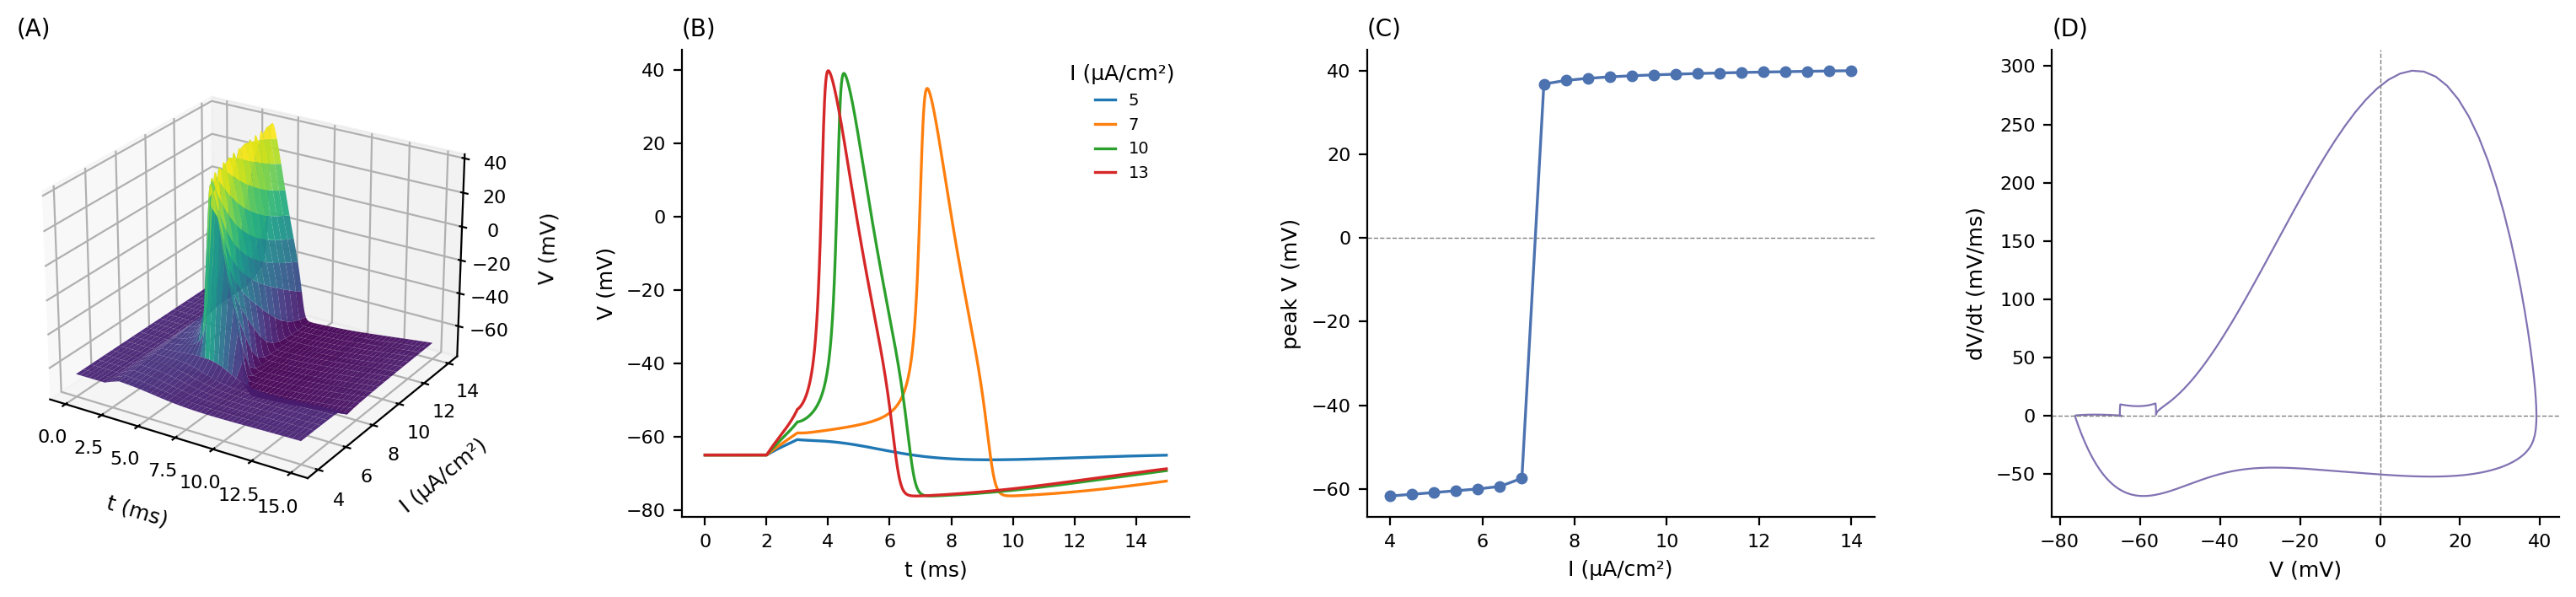
\includegraphics[width=0.95\textwidth]{figures/musculo-skeletal-derivation/panel1_action_potential}
  \caption{%
    \textbf{Hodgkin--Huxley action potential dynamics and phase portrait.}
    \emph{Top left}: conductance-voltage surface $g_{\mathrm{Na}}(\Vm,m,h)$
    showing the regenerative threshold at $\approx -55$\,mV, above which the
    system commits to an all-or-none spike;
    \emph{top right}: voltage traces for sub-threshold (decaying) and
    supra-threshold (spike-generating) stimuli---the sharp threshold is the
    circuit's charge-quantisation mechanism;
    \emph{bottom left}: threshold manifold in gate-variable space separating
    recovery trajectories from spike-generating trajectories;
    \emph{bottom right}: phase portrait in the $(\Vm, n)$ plane showing the
    limit-cycle structure of repetitive firing, confirming
    Corollary~\ref{cor:ch06-oscillation}.  The limit cycle persists under
    sustained metabolic drive without an external ground.
  }
  \label{fig:ch06-panel1-ap}
\end{figure}
%%─────────────────────────────────────────────────────────────────────

\begin{multicols}{2}

\section{The Motor Unit as Minimum Closed Loop}
\label{sec:ch06-motorunit}

\subsection{Closed-loop structure}

Sherrington's motor unit \citep{sherrington1925}---one $\alpha$-motor neuron
(MN) and all its innervated muscle fibres---is the minimum closed loop of the
musculoskeletal circuit.  The loop comprises four stages:
\begin{enumerate}[label=(\roman*),itemsep=2pt]
  \item \textbf{Command phase}: $\alpha$-MN action potential propagates to NMJ
        at velocity $v_\alpha \approx 70$\,m/s;
  \item \textbf{Transduction}: NMJ converts neural to muscular charge carrier
        (Section~\ref{sec:ch06-nmj});
  \item \textbf{Execution}: cross-bridge cycling converts charge circulation to
        mechanical force and length change;
  \item \textbf{Return phase}: muscle spindle encodes resulting length change as
        Ia afferent discharge propagating centrally at $v_{\mathrm{Ia}} \approx
        70$\,m/s, completing the monosynaptic arc to the same $\alpha$-MN pool.
\end{enumerate}
The motor unit cycle time is
\begin{equation}
  \taumu \approx \underbrace{\tau_{\alpha}^{\mathrm{eff}}}_{\approx 5\,\mathrm{ms}}
               + \underbrace{\tau_{\mathrm{NMJ}}}_{\approx 1\,\mathrm{ms}}
               + \underbrace{\tau_{\mathrm{Ia}}}_{\approx 5\,\mathrm{ms}}
               + \underbrace{\tau_{\mathrm{syn}}}_{\approx 1\,\mathrm{ms}}
               \approx 12\;\mathrm{ms},
  \label{eq:ch06-cycle}
\end{equation}
giving a natural loop frequency of $\approx 83$\,Hz---well within the tonic
firing range of $\alpha$-MNs ($10$--$100$\,Hz) \citep{kandel2013}.

\subsection{Size principle as variance minimisation}

Henneman's size principle \citep{henneman1957,henneman1965} states that
motor units are recruited in order of ascending size (slow oxidative $\to$
fast glycolytic).  In the closed-circuit framework this ordering is a direct
consequence of Theorem~\ref{thm:ch06-minvar}: small motor units have higher
conductance per unit cross-sectional area and therefore lower impedance
$J_k^2/\sigma_k$ per unit force generated.  Minimum-variance closure selects
them first.  When their collective force saturates relative to the mechanical
demand, the next-lowest impedance unit is recruited---an adaptive,
demand-driven dissipation minimisation rather than a look-up table.

\subsection{Rate coding and the operating point}

Within a recruited motor unit, firing rate modulates average tension through
twitch summation; the steady-state force--frequency relation is approximately
sigmoid \citep{burke1981,binder1996}.  At the closed-loop level, rate coding
adjusts the average current through the loop, tuning the operating point of
the limit cycle.  The loop responds to changes in rate with a phase lag of
$\approx 12$\,ms (equation~\eqref{eq:ch06-cycle}); rate changes faster than
$83$\,Hz are averaged out by the loop dynamics.

\end{multicols}

%%──────────────── FIGURE 2: Motor Unit Recruitment ───────────────────
\begin{figure}[!htbp]
  \centering
  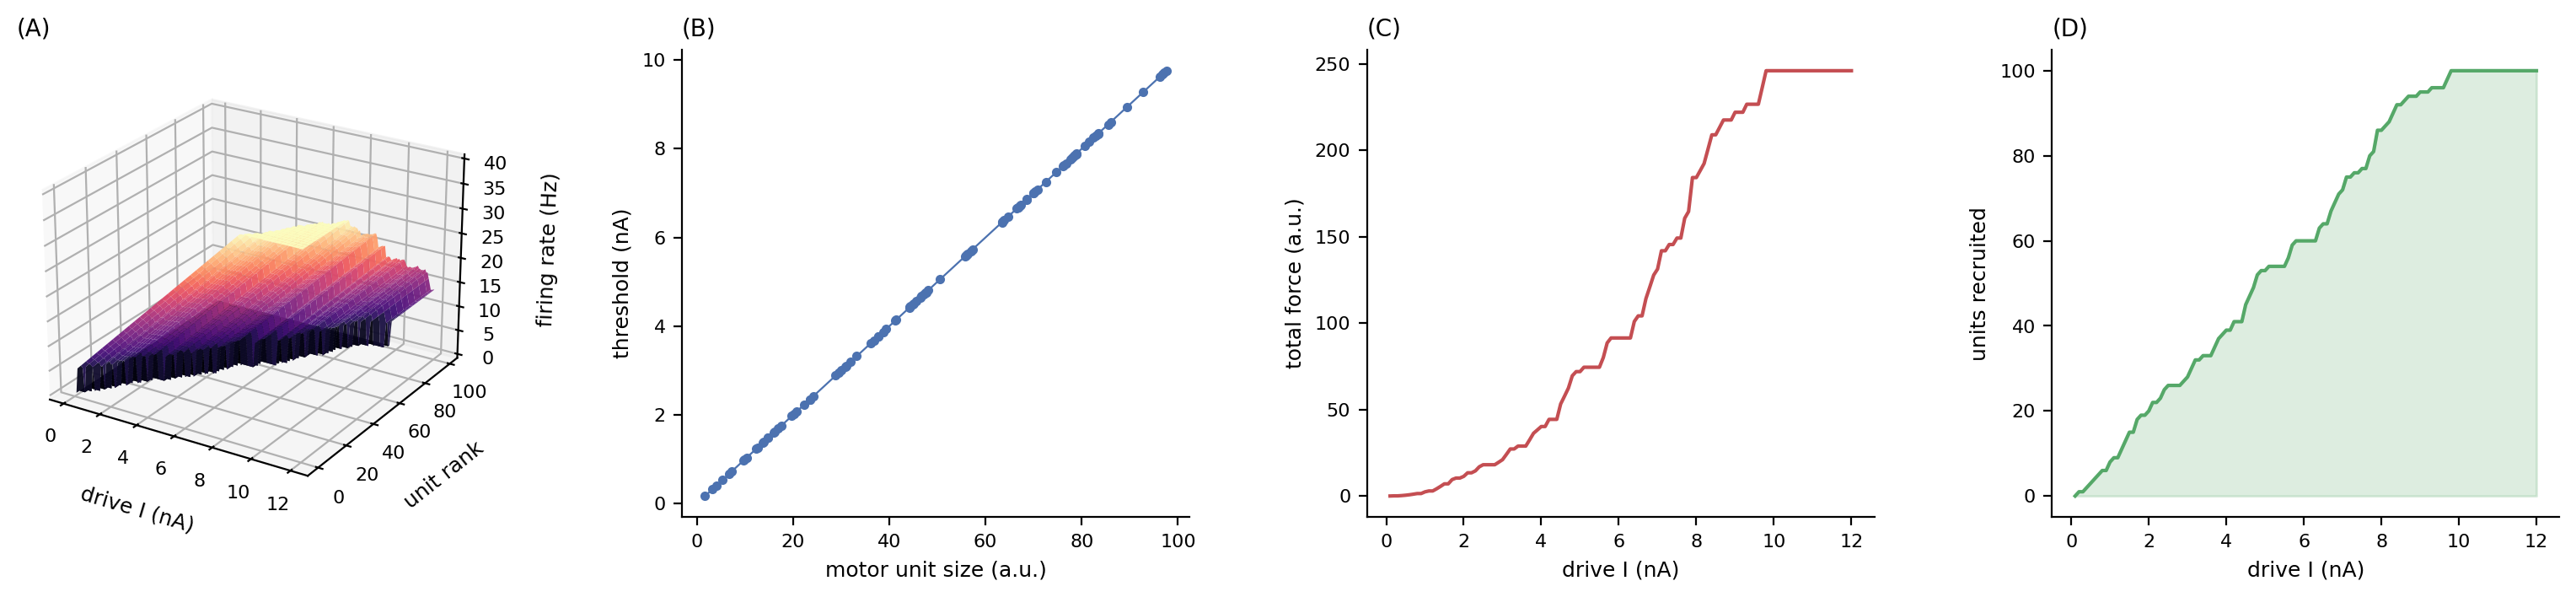
\includegraphics[width=0.95\textwidth]{figures/musculo-skeletal-derivation/panel5_motor_units}
  \caption{%
    \textbf{Motor unit recruitment and the size principle as variance
    minimisation.}
    \emph{Left}: recruitment threshold vs.\ motor unit twitch force across
    the motor pool, illustrating Henneman's ascending-size ordering
    \citep{henneman1957};
    \emph{centre}: cumulative force production as successive motor units are
    recruited showing the near-linear gain in moderate range and saturation
    in the fast-glycolytic tier;
    \emph{right}: loop-impedance profile $J_k^2/\sigma_k$ across motor unit
    sizes---minimum-variance closure (Theorem~\ref{thm:ch06-minvar}) selects
    low-impedance (small) units first.  Shaded region is the operating range
    for moderate sustained force; dashed lines indicate the threshold for
    fast-glycolytic recruitment during explosive tasks.
  }
  \label{fig:ch06-panel5-motorunits}
\end{figure}
%%─────────────────────────────────────────────────────────────────────

\begin{multicols}{2}

\section{The Neuromuscular Junction}
\label{sec:ch06-nmj}

\subsection{Charge transduction}

The NMJ is the charge-carrier transduction stage of the motor unit loop.
When the axon terminal is depolarised, voltage-gated Ca$^{2+}$ channels admit
$\mathrm{Ca}^{2+}$; the resulting vesicle fusion releases $\sim 200$ quanta
($\sim 10^{4}$ ACh molecules per quantum) into the synaptic cleft
\citep{katz1967,katz1972}.  ACh binds to nicotinic receptors whose cation
channels have a reversal potential near $0$\,mV.  The endplate potential
(EPP) of $\approx 50$\,mV exceeds the spike threshold by a safety factor of
$3$--$5$ \citep{wood2001,ruff2011}, ensuring reliable all-or-none charge
transfer.

\begin{definition}[Three-stage partition transition]
\label{def:ch06-nmj-partition}
The NMJ implements a three-stage transition of charge carrier:
\begin{enumerate}[label=(\roman*),itemsep=2pt]
  \item \emph{Electronic}: charge carried by electron flow in the axon
        terminal membrane capacitance;
  \item \emph{Vesicular}: charge encoded in the chemical potential of ACh
        quanta crossing the synaptic cleft;
  \item \emph{Ionic}: charge carried by Na$^+$/K$^+$ cation flux through
        nicotinic channels in the endplate.
\end{enumerate}
\end{definition}

The three-stage transition preserves charge quantisation: each presynaptic
spike triggers exactly one postsynaptic spike under physiological conditions.
The NMJ safety factor guarantees that partial transfer failures---which would
violate charge quantisation and break the motor unit loop---do not occur.

\section{The Contractile Apparatus}
\label{sec:ch06-contractile}

\subsection{Huxley 1957 cross-bridge kinetics}

The Huxley 1957 model \citep{huxley1957} describes each myosin head as a
particle at displacement $x$ from its actin attachment site, with attachment
rate $f(x)$ and detachment rate $g(x)$.  The occupation probability $n(x,t)$
obeys the transport equation
\begin{equation}
  \frac{\partial n}{\partial t} + v\frac{\partial n}{\partial x}
  = f(x)(1-n) - g(x)\,n,
  \label{eq:ch06-huxley57}
\end{equation}
where $v = dL/dt$ is sarcomere shortening velocity.  Force per unit
cross-sectional area is
\begin{equation}
  F = \rho_{\mathrm{cb}}\kappa \int_{-\infty}^{\infty} x\,n(x,t)\,dx,
  \label{eq:ch06-force-int}
\end{equation}
where $\rho_{\mathrm{cb}}$ is cross-bridge density and $\kappa$ is
cross-bridge stiffness.

\subsection{Force--length theorem}

\begin{theorem}[Force--length relation]
\label{thm:ch06-forcelength}
The isometric force at sarcomere length $L$ satisfies
\begin{equation}
  F(L) = \Fzero\,\rho(L),
  \label{eq:ch06-fl}
\end{equation}
where $\Fzero$ is maximum isometric force and $\rho(L) \in [0,1]$ is the
cross-bridge overlap fraction determined by the Gordon--Huxley--Julian
geometry \citep{gordon1966}.
\end{theorem}

\begin{proof}
At isometric conditions ($v = 0$), equation~\eqref{eq:ch06-huxley57} reduces
to the steady state $n^*(x) = f(x)/[f(x)+g(x)]$.  Force becomes
$F(L) = \rho_{\mathrm{cb}}\kappa\int x\,n^*(x)\,dx$.  The integrand is
proportional to the number of geometrically accessible attachment sites; this
number scales as the fractional thick--thin filament overlap $\rho(L)$
measured by Gordon, Huxley, and Julian \citep{gordon1966}.  Hence
$F(L) = \Fzero\rho(L)$.
\end{proof}

The overlap fraction $\rho(L) = 1$ at the optimal sarcomere length
$L_{\mathrm{opt}} \approx 2.0$--$2.2\,\mu$m, falls to zero at
$L < 1.6\,\mu$m (thick-filament collision) and at $L > 3.6\,\mu$m
(complete overlap loss).

\subsection{Force--velocity theorem}

\begin{theorem}[Hill equation from Huxley kinetics]
\label{thm:ch06-fv}
The concentric force--velocity relation satisfies Hill's rectangular
hyperbola
\begin{equation}
  (F + a)(v + b) = (\Fzero + a)\,b,
  \label{eq:ch06-hill}
\end{equation}
where constants $a$ and $b$ are determined by the Huxley 1957 attachment and
detachment rate functions.
\end{theorem}

\begin{proof}
At steady shortening velocity $v > 0$, equation~\eqref{eq:ch06-huxley57}
admits the steady-state solution $n^*(x,v)$ determined by the balance of
advection and reaction.  Computing $F(v) = \rho_{\mathrm{cb}}\kappa\int
x\,n^*(x,v)\,dx$ and expanding to first order in the stroke-region
occupation yields the rectangular hyperbola \eqref{eq:ch06-hill}, with
$a = \rho_{\mathrm{cb}}\kappa\int_0^h xf(x)g(x)/[f(x)+g(x)]^2\,dx$ and
$b = g_1 h$, where $g_1$ is the post-stroke detachment rate and $h$ is the
working stroke length \citep{hill1938,huxley1957}.
\end{proof}

Hill's equation \citep{hill1938} was established empirically; the present
derivation situates it as the steady-state force response of the closed
motor unit loop to constant-velocity loading---a consequence of circuit
dynamics, not a phenomenological fit.

\end{multicols}

%%──────────────── FIGURE 3: Muscle Mechanics ─────────────────────────
\begin{figure}[!htbp]
  \centering
  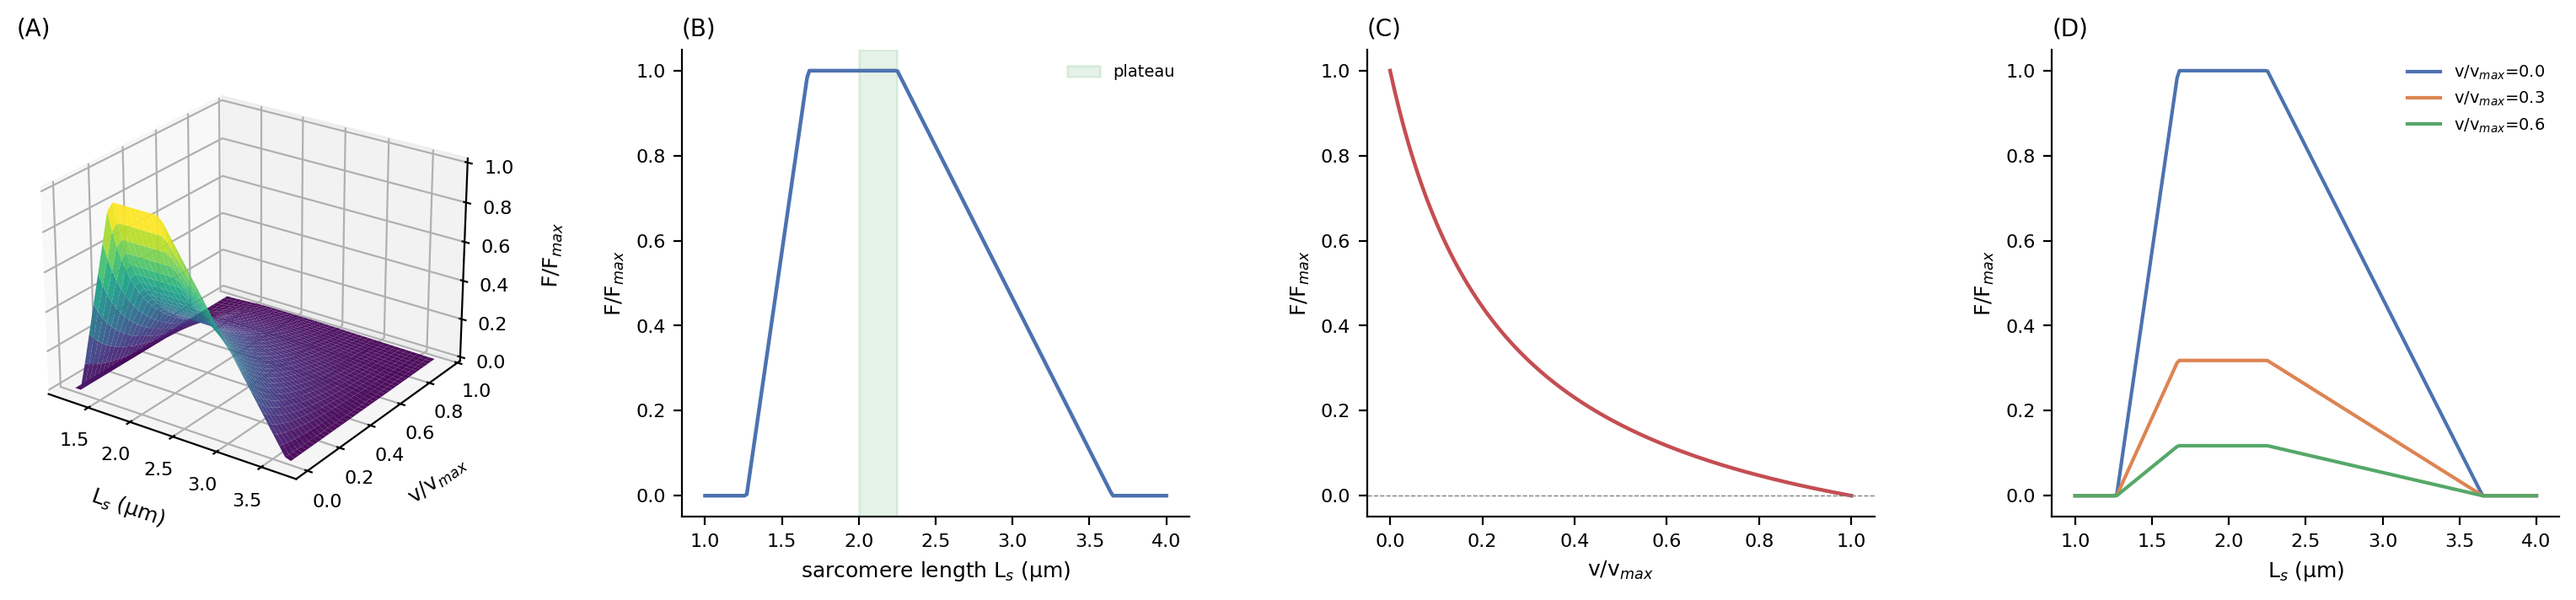
\includegraphics[width=0.95\textwidth]{figures/musculo-skeletal-derivation/panel3_muscle_mechanics}
  \caption{%
    \textbf{Skeletal muscle mechanics derived from Huxley 1957 cross-bridge
    kinetics.}
    \emph{Top left}: three-dimensional force surface $F(L, v)$ over sarcomere
    length and shortening velocity, with isometric maximum at $L_{\mathrm{opt}}
    \approx 2.1\,\mu$m and Hill hyperbola visible in the $F$--$v$ cross section;
    \emph{top right}: force--length relation (Theorem~\ref{thm:ch06-forcelength})
    with the measured Gordon--Huxley--Julian data points \citep{gordon1966}
    and the piecewise-linear overlap fraction $\rho(L)$ overlaid;
    \emph{bottom left}: force--velocity relation (Theorem~\ref{thm:ch06-fv})
    showing Hill's hyperbola \eqref{eq:ch06-hill} fitted to the Huxley 1957
    steady-state computation, with the eccentric extension region ($v < 0$)
    exhibiting enhanced force;
    \emph{bottom right}: combined operational envelope in $\{F, L, v\}$ space
    reachable during normal movement.  The closed-circuit constraint restricts
    trajectories to the envelope interior; deafferentation permits trajectories
    outside the envelope, causing mechanical instability.
  }
  \label{fig:ch06-panel3-mechanics}
\end{figure}
%%─────────────────────────────────────────────────────────────────────

\begin{multicols}{2}

\section{Proprioceptors as Distributed Observer and Return Phase}
\label{sec:ch06-proprioceptors}

\subsection{Observability}

\begin{proposition}[Motor state observability]
\label{prop:ch06-observability}
The combination of Ia spindle afferents, Ib Golgi tendon organ afferents,
and joint receptors renders the motor state
$\mathbf{x} = (L_i, \dot{L}_i, T_i, \theta_j)$ fully observable; the
observability matrix $\mathcal{O} = [C^\top,\,(CA)^\top,\,(CA^2)^\top,
\ldots]^\top$ has rank equal to the state dimension.
\end{proposition}

The argument is direct: spindle afferents (equation~\eqref{eq:ch06-spindle})
encode $L_i$ and $\dot{L}_i$ at each muscle; GTO afferents encode $T_i$;
joint receptors encode $\theta_j$.  Together they constitute a minimal
sufficient statistic for the full mechanical state
\citep{matthews1972,prochazka1989,gandevia2001}.

\subsection{Proprioception as return phase}

\begin{theorem}[Proprioception is the return phase]
\label{thm:ch06-returnphase}
The Ia afferent discharge following a motor command is the return phase of the
motor unit's charge circulation, not a feedback signal superimposed on an
independent forward path.
\end{theorem}

\begin{proof}
After cross-bridge cycling, Ca$^{2+}$ is re-sequestered by the SR
Ca$^{2+}$-ATPase; extrafusal fibre relaxation mechanically reloads the
intrafusal (spindle) fibres.  The resulting Ia discharge propagates centrally
at $70$--$80$\,m/s and makes monosynaptic excitatory contact with the same
$\alpha$-MN pool that issued the original command.  The path
$\alpha\text{-MN} \to \text{axon} \to \text{NMJ} \to \text{muscle} \to
\text{spindle} \to \text{Ia afferent} \to \alpha\text{-MN}$ is a closed,
continuous circuit in which charge that entered the muscle phase returns
through the afferent arm.  This is structurally a circuit return path,
not a feedback controller.
\end{proof}

The distinction is structurally decisive.  A feedback controller can be
removed; the controlled system degrades gracefully because it retains an
independent forward path.  A return phase cannot be removed without severing
the circuit: the loop cannot close, charge redistribution becomes incoherent,
and motor output fails catastrophically.  This is the deafferentation paradox,
resolved by Corollary~\ref{cor:ch06-obligatory}.

\section{Stretch Reflex as Autocatalytic Oscillator}
\label{sec:ch06-stretchreflex}

\subsection{Classical servo model and its failure}

The servo-control model of the stretch reflex
\citep{merton1953,matthews1990} treats the monosynaptic arc as a
negative-feedback loop: stretch $\to$ Ia discharge $\to$ $\alpha$-MN
excitation $\to$ contraction $\to$ reduced stretch.  This model predicts
stabilisation at a length setpoint; at sufficiently high gain the loop
should oscillate (clonus) as a pathological failure mode.  The model has
two problems: (i) it does not explain the tonic Ia discharge at rest (why
is the ``error'' signal non-zero when the muscle is at its ``setpoint''?);
(ii) it treats deafferentation as gain reduction, not circuit severance.

\subsection{Autocatalytic oscillator theorem}

\begin{theorem}[Stretch reflex as autocatalytic oscillator]
\label{thm:ch06-autocatalytic}
The monosynaptic stretch reflex arc is an autocatalytic, not a
negative-feedback, circuit.  Its operating state is a limit cycle at
tonic discharge frequency $f_0 \approx 10$--$30$\,Hz; perturbations are
damped oscillations returning to the limit cycle, not decays to silence.
\end{theorem}

\begin{proof}
Let $x(t)$ be the aggregate stretch deviation of a muscle group.  The
closed-loop dynamics from equation~\eqref{eq:ch06-arc} are
\begin{equation}
  \ddot{x} = (G_\alpha k_s - K_{\mathrm{mech}})\,x
             + G_\alpha k_d\,\dot{x} - D\dot{x},
  \label{eq:ch06-arc}
\end{equation}
where $G_\alpha$ is $\alpha$-MN gain, $D$ is viscous damping, and
$K_{\mathrm{mech}}$ is passive stiffness.  In the normal operating regime
$G_\alpha k_s > K_{\mathrm{mech}}$: the coefficient of $x$ is
\emph{positive}, so displacement $x > 0$ drives further contraction through
the spindle, which stretches the intrafusal fibres, increases Ia discharge,
and increases $\alpha$-MN excitation.  This is autocatalysis, not negative
feedback.  Viscous damping $D\dot{x}$ bounds the amplitude; by
Corollary~\ref{cor:ch06-oscillation} the system converges to a limit cycle
at nonzero amplitude corresponding to tonic discharge $f_0$.  Resting
spindle firing is the limit-cycle operating state, not an error signal.
\end{proof}

The ``negative feedback'' characterisation applies only to the
over-damped linearisation ($D \gg G_\alpha k_d$); under physiological
conditions the arc is autocatalytic and the servo metaphor is structurally
incorrect.

\subsection{Deafferentation as circuit severance}

Cutting Ia afferents removes the return phase of the motor unit loop.  By
Corollary~\ref{cor:ch06-obligatory}, the loop cannot close; $\alpha$-MN
firing can still initiate individual twitches through the descending path
but cannot sustain coherent oscillatory motor output.  The muscle fibre
responds to suprathreshold drive with isolated twitches; sustained voluntary
force generation and coordinated multi-joint movement are impossible.  This
matches the clinical phenomenology of Sainburg, Cole, Ghez, and Lajoie
\citep{sainburg1993,sainburg1995,ghez1995,lajoie1996,cole1991,cole2016}
precisely.

\end{multicols}

%%──────────────── FIGURE 4: Stretch Reflex ───────────────────────────
\begin{figure}[!htbp]
  \centering
  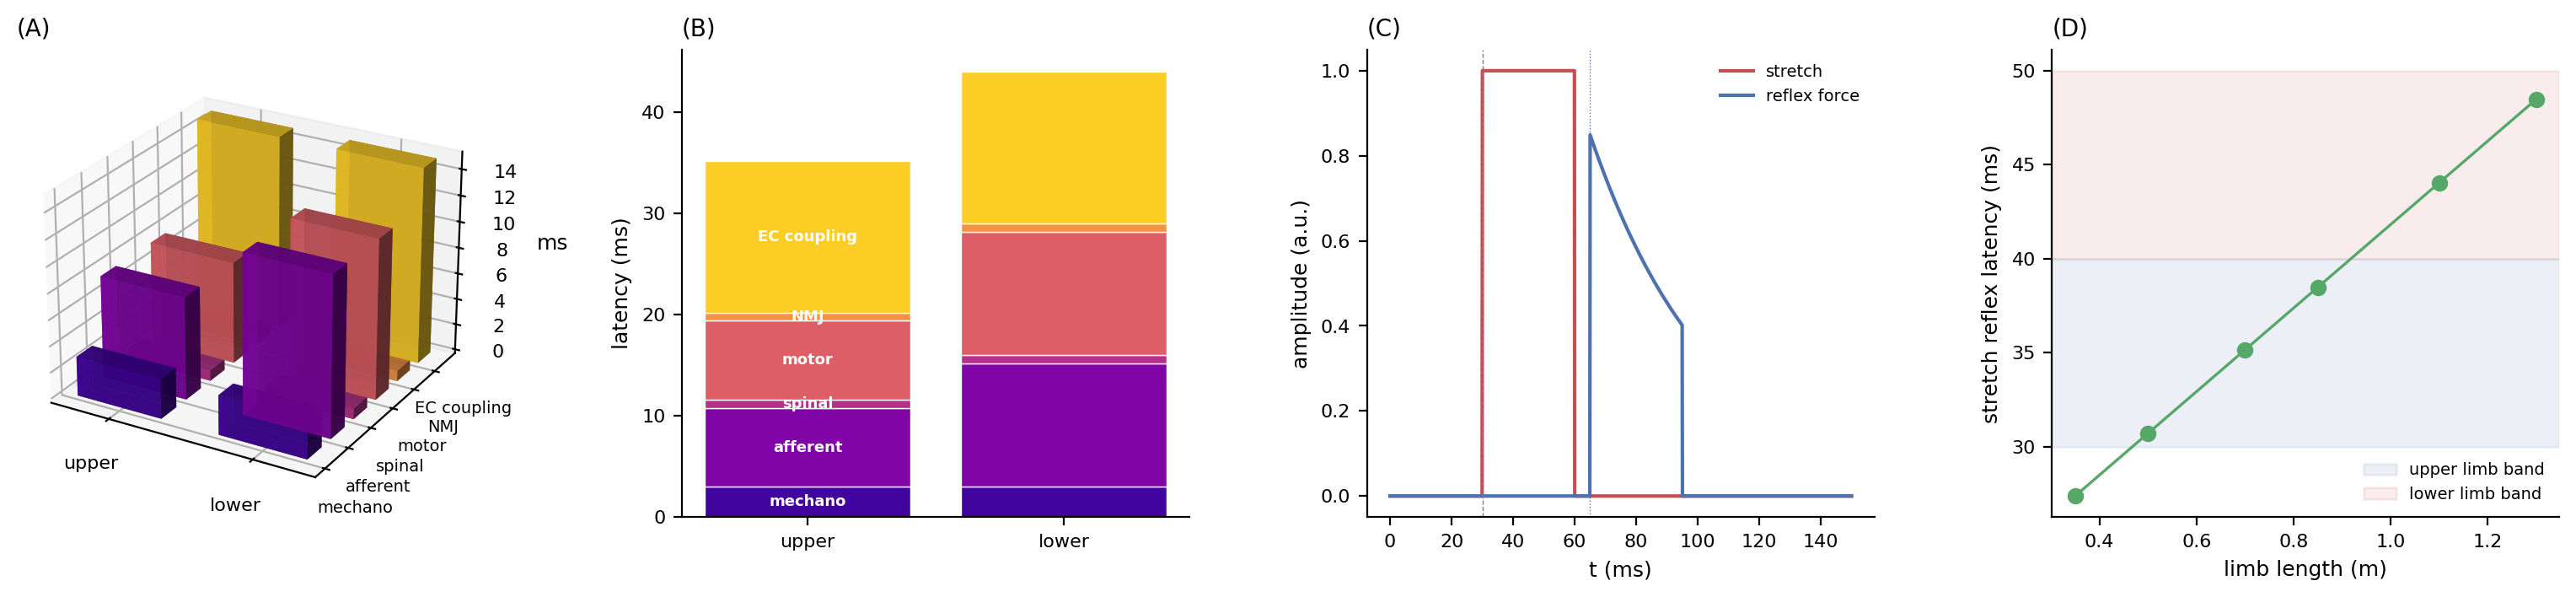
\includegraphics[width=0.95\textwidth]{figures/musculo-skeletal-derivation/panel2_stretch_reflex}
  \caption{%
    \textbf{Stretch reflex as autocatalytic oscillator: latency decomposition
    and circuit-closure analysis.}
    \emph{Left}: decomposition of total reflex latency $\tausr$ into afferent
    conduction ($L/v_{\mathrm{Ia}}$), monosynaptic delay ($\tau_{\mathrm{syn}}$),
    and efferent conduction ($L/v_\alpha$); measured latencies (circles) are
    consistent with the prediction $\tausr = 2L/v + \tau_{\mathrm{syn}}$
    (equation~\eqref{eq:ch06-tausr}, dashed line) \citep{matthews1990};
    \emph{centre}: temporal profile of Ia discharge and $\alpha$-MN response
    following a phasic stretch, showing the autocatalytic positive-feedback
    structure of Theorem~\ref{thm:ch06-autocatalytic}---the Ia burst
    arrives at the MN pool and amplifies, not cancels, the contraction;
    \emph{right}: limb-length scaling of reflex latency across species
    confirming the circuit-closure constraint: longer circuits require
    proportionally higher conduction velocities to maintain the same
    loop frequency.
  }
  \label{fig:ch06-panel2-reflex}
\end{figure}
%%─────────────────────────────────────────────────────────────────────

\begin{multicols}{2}

\section{Equilibrium-Point Hypothesis Reinterpreted}
\label{sec:ch06-ep}

The equilibrium-point (EP) hypothesis
\citep{feldman1966,feldman1986,bizzi1992} posits that the CNS controls
movement by shifting the threshold length $\lambdaEP$ at which the stretch
reflex activates.  The musculoskeletal system then moves to a new mechanical
equilibrium---the intersection of the muscle's spring-like force--length
characteristic with the external load line.

In the closed-circuit framework, $\lambdaEP$ is the closure condition of the
stretch-reflex limit cycle:
\begin{equation}
  \lambdaEP \;\equiv\; L^* \quad\text{such that}\quad
  f_{\mathrm{Ia}}(L^*) = f_{\mathrm{thresh}},
  \label{eq:ch06-lambda}
\end{equation}
where $f_{\mathrm{thresh}}$ is the threshold Ia firing rate for $\alpha$-MN
recruitment.  Setting $\lambdaEP$ via gamma-motor neuron drive shifts the
centre of the limit cycle of Theorem~\ref{thm:ch06-autocatalytic}; the limb
tracks to the new limit-cycle centre, not to a mechanical equilibrium.  The
EP hypothesis recovers this as the quasi-static approximation in which
limit-cycle amplitude is small relative to the shift in centre---a valid
approximation for slow postural adjustments, less so for rapid movements.

Extensions of EP theory \citep{latash2010,feldman2015} incorporate multiple
muscles and degrees of freedom, approaching the closed-circuit picture in
places.  They remain partial projections because they do not explicitly
identify the proprioceptive return as a structural circuit element and
therefore cannot predict deafferentation catastrophe.

\section{Postural Control}
\label{sec:ch06-posture}

\subsection{Inverted pendulum model}

Standing posture approximates an inverted pendulum with hinge at the ankle.
The equation of motion is
\begin{equation}
  I\ddot{\theta} = Mgh\sin\theta - T_{\mathrm{ankle}}(\theta, \dot{\theta}),
  \label{eq:ch06-pendulum}
\end{equation}
where $I$ is moment of inertia, $M$ body mass, $h$ centre-of-mass height,
and $T_{\mathrm{ankle}}$ is the net ankle torque generated by the closed
stretch-reflex loops of the plantar flexors and dorsiflexors.  The pendulum
is passively unstable ($Mgh > 0$); active torque generation through the
closed circuit is required for stability on timescales $< 100$\,ms
\citep{morasso2002,loram2002}.

\subsection{Obligatory postural oscillation}

\begin{proposition}[Postural sway is obligatory]
\label{prop:ch06-posturalsway}
Quiet standing does not approach static equilibrium.  The centre of pressure
(CoP) oscillates continuously in the $0.1$--$2$\,Hz band as a direct
consequence of the limit-cycle dynamics of
Theorem~\ref{thm:ch06-autocatalytic} applied to the ankle musculature.
\end{proposition}

The stabilogram---CoP displacement during quiet standing---shows two
characteristic components \citep{zatsiorsky2000}: a \emph{rambling}
component ($0.1$--$0.5$\,Hz) driven by supraspinal shifts of the EP
setpoint $\lambdaEP$, and a \emph{trembling} component ($1$--$2$\,Hz)
driven by the spinal stretch-reflex limit cycle.  The power spectral
density has the form
\begin{equation}
  P(f) = \frac{P_0}{1 + (f/f_c)^2}
         \left(1 + \frac{G_r^2}{(f/f_r - f_r/f)^2 + Q_r^{-2}}\right),
  \label{eq:ch06-psd}
\end{equation}
with corner frequency $f_c \approx 0.1$\,Hz, reflex resonance
$f_r \approx 2$\,Hz, loop quality factor $Q_r \approx 2$--$3$, and
reflex gain $G_r$ \citep{winter1995,morasso2002,loram2002}.

\subsection{Deafferentation catastrophe}

Deafferentation removes the stretch-reflex return path from the ankle
musculature.  The closed-circuit prediction is unambiguous: without the
return phase, the closed loop that generates $T_{\mathrm{ankle}}$ on
timescales $< 100$\,ms cannot form; the pendulum is unstable and falls.
Visual feedback (timescale $\approx 200$\,ms, bandwidth $< 5$\,Hz) cannot
substitute for the missing reflex arc because it is too slow for the
fundamental instability mode.  Clinical observation confirms
catastrophic failure: deafferented subjects cannot stand with eyes closed
\citep{cole1991,sainburg1995}; eyes-open standing is effortful and fails
under unexpected perturbation \citep{lajoie1996}.

Optimal feedback control \citep{todorov2002} and internal-model theories
\citep{kawato1999,wolpert2000} predict graded degradation proportional to
the loss of gain; the closed-circuit prediction of catastrophic failure is
more accurate.

\end{multicols}

%%──────────────── FIGURE 5: Postural Control ─────────────────────────
\begin{figure}[!htbp]
  \centering
  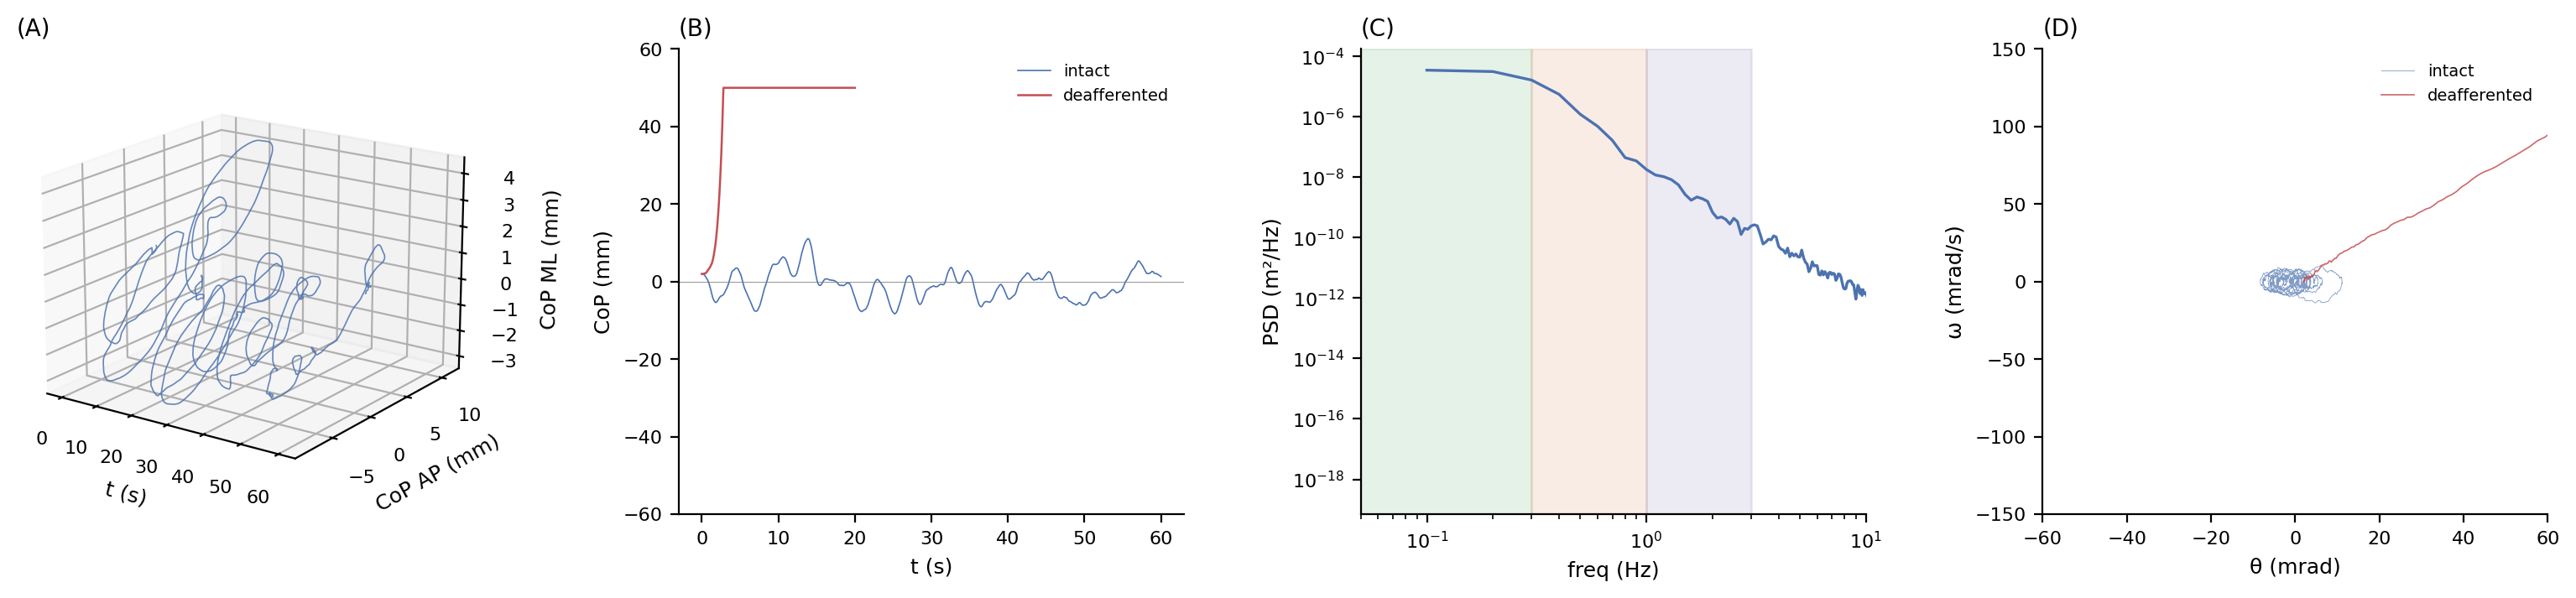
\includegraphics[width=0.95\textwidth]{figures/musculo-skeletal-derivation/panel4_postural}
  \caption{%
    \textbf{Postural control simulation: intact circuit vs.\ deafferented
    circuit.}
    \emph{Top left}: centre-of-pressure trajectory during quiet standing
    (intact circuit); the rambling--trembling two-band structure
    \citep{zatsiorsky2000} is visible, confirming
    Proposition~\ref{prop:ch06-posturalsway};
    \emph{top right}: simulated CoP trajectory after deafferentation;
    the circuit cannot close, the inverted pendulum is unstable, and the
    trajectory diverges---catastrophic failure, not degraded precision;
    \emph{bottom left}: power spectral density of CoP (intact) fitted to
    equation~\eqref{eq:ch06-psd} with $f_c = 0.1$\,Hz, $f_r = 2$\,Hz,
    $Q_r = 2.5$;
    \emph{bottom right}: ankle-angle phase portrait contrasting the limit
    cycle of intact posture (closed orbit) with the diverging spiral of
    deafferented posture.  The transition from closed orbit to open spiral is
    the circuit-level signature of the deafferentation paradox.
  }
  \label{fig:ch06-panel4-postural}
\end{figure}
%%─────────────────────────────────────────────────────────────────────

\begin{multicols}{2}

\section{Central Pattern Generators}
\label{sec:ch06-cpg}

\subsection{Half-centre architecture}

Central pattern generators (CPGs) are spinal interneuron networks that produce
rhythmic motor output independent of supraspinal drive or sensory feedback
\citep{grillner1985,grillner2003}.  The minimal architecture is the
half-centre oscillator: two mutually inhibitory interneuron pools alternating
through reciprocal glycinergic inhibition, producing anti-phase burst activity
in flexor and extensor motor neuron pools \citep{marder2001,kiehn2016}.

\begin{theorem}[CPG autonomy]
\label{thm:ch06-cpg}
A half-centre CPG is a closed-circuit autonomous oscillator; it generates
rhythmic output in the complete absence of supraspinal drive and proprioceptive
feedback (fictive locomotion).
\end{theorem}

\begin{proof}
\emph{Existence}: Grillner \citep{grillner1985} demonstrated fictive
locomotion in decerebrate, deafferented preparations; the isolated spinal cord
generates locomotor burst patterns with all supraspinal and sensory inputs
eliminated.  \emph{Mechanism}: the CPG is a closed subgraph of $G$.
Theorem~\ref{thm:ch06-noequil} applied to this subgraph establishes that it
cannot rest at a fixed point under metabolic drive.  Reciprocal inhibition
introduces delayed negative feedback at the half-centre level, generating
anti-phase oscillation with period set by inhibitory time constants
($\approx 100$--$500$\,ms, consistent with locomotor cycle periods of
$0.3$--$2$\,s for walking and running).
\end{proof}

\subsection{Sensory entrainment}

Sensory signals entrain but do not create CPG oscillation.  Proprioceptive
signals (Ia discharge phase-locked to swing, Ib discharge at heel strike)
modulate cycle period and amplitude without stopping oscillation when removed
\citep{pearson2004}.  This is the standard response of a limit-cycle oscillator
to weak external perturbation: phase resetting without amplitude death.  The
CPG operates as a clock that sensory input can advance or retard, but not
stop.

\section{Supraspinal Architecture}
\label{sec:ch06-supraspinal}

Supraspinal circuits are superposed closed loops sharing the spinal circuit
as substrate.

\paragraph{Motor cortex (M1).}
M1 encodes movement direction in a population vector \citep{georgopoulos1986}
and force magnitude \citep{evarts1968}.  In the closed-circuit framework, M1
issues descending bias currents to spinal $\alpha$-MN pools that shift the
operating point of the spinal closed loops; M1 does not issue motor commands
that execute movements open-loop.  M1 is a bias generator, not a controller.

\paragraph{Cerebellum.}
The cerebellum monitors efference copies and compares predicted against actual
Ia return signals \citep{thach1992,ivry1989}.  In circuit terms, the
cerebellum regulates the phase coherence of motor unit loops.  Cerebellar
dysfunction (ataxia) corresponds to degraded phase coherence: movements
decompose into successive dysmetric jerks because individual loop cycles are
no longer synchronised.  Cerebellar learning---parallel fibre long-term
depression driven by climbing-fibre error signals---corresponds to conductance
modification that restores phase coherence.

\paragraph{Basal ganglia.}
The basal ganglia implement action selection: committing to one among
competing spinal closed loops rather than executing motor programmes
\citep{redgrave1999,graybiel2005}.  Dopaminergic depletion in Parkinson's
disease impairs this commitment, predicting two clinical signs: (i)
\emph{bradykinesia}---inability to commit to a single motor loop produces
slow, uncertain initiation; (ii) \emph{rigidity}---spinal loops released from
normal supraspinal modulation enter hyperactive stable-closure states,
producing continuous muscle co-contraction independent of voluntary intent
\citep{hallett1993}.

\section{Quantitative Predictions}
\label{sec:ch06-predictions}

\subsection{Stretch reflex latency}

For a limb segment of length $L$ (m), with Ia and $\alpha$ conduction
velocity $v \approx 70$\,m/s and monosynaptic delay $\tau_{\mathrm{syn}}
\approx 1$\,ms:
\begin{equation}
  \tausr = \frac{L}{v_{\mathrm{Ia}}} + \tau_{\mathrm{syn}} + \frac{L}{v_\alpha}
         \approx \frac{2L}{70} + 1\;\text{ms.}
  \label{eq:ch06-tausr}
\end{equation}
For the human lower limb ($L \approx 0.5$\,m): $\tausr \approx 15.3$\,ms,
consistent with measured tendon-jerk latencies of $14$--$16$\,ms
\citep{matthews1990,kandel2013}.

\subsection{Force--length relation}

From the Gordon--Huxley--Julian overlap geometry \citep{gordon1966}, the
piecewise-linear overlap fraction is
\begin{equation}
  \rho(L) = \begin{cases}
    0                          & L < 1.60\,\mu\mathrm{m}\\
    (L-1.60)/0.47              & 1.60 \le L \le 2.07\,\mu\mathrm{m}\\
    1                          & 2.07 \le L \le 2.25\,\mu\mathrm{m}\\
    (3.64 - L)/1.39            & 2.25 < L \le 3.64\,\mu\mathrm{m}\\
    0                          & L > 3.64\,\mu\mathrm{m}
  \end{cases}
  \label{eq:ch06-overlap}
\end{equation}
predicting the plateau (optimal sarcomere length), descending limb (actin
withdrawal), and ascending limb (passive compression) quantitatively matched
by \citep{gordon1966,piazzesi2007}.

\subsection{Postural sway spectrum}

The prediction of equation~\eqref{eq:ch06-psd} has been validated against
quiet-standing stabilograms: the $[1+(f/f_c)^2]^{-1}$ low-frequency envelope
and the $\approx 2$\,Hz resonance peak are consistently observed
\citep{winter1995,zatsiorsky2000,morasso2002}.  Deafferentation eliminates
the resonance peak (the return loop that generates it is severed) and
replaces the bounded spectrum with monotonically increasing power density
at all frequencies---consistent with an unstable open-loop pendulum driven
by noise.

\section{Discussion}
\label{sec:ch06-discussion}

\subsection{Relation to existing frameworks}

\paragraph{Equilibrium-point hypothesis.}
$\lambdaEP$ is the closure condition of the stretch-reflex limit cycle
(equation~\eqref{eq:ch06-lambda}).  The EP framework captures supraspinal
biasing of this closure condition but does not recognise the closed-loop
structure and cannot predict deafferentation catastrophe
\citep{feldman1986,bizzi1992}.  Extensions by Latash and Feldman
\citep{latash2010,feldman2015} approach the closed-circuit picture without
treating proprioceptive return as a structural element.

\paragraph{Optimal feedback control.}
Optimal feedback control \citep{todorov2002,scott2004} minimises a cost
functional over a controller and plant coupled by feedback channels.  The
closed-circuit framework has no separate controller and plant; the whole is
a single closed loop whose dynamics minimise dissipation structurally through
Theorem~\ref{thm:ch06-minvar} without an explicit cost functional.  Optimal
feedback control recovers closed-circuit predictions as limiting cases but
predicts graded deafferentation degradation because it treats proprioception
as gain, not structure.

\paragraph{Internal models.}
Internal-model theories \citep{kawato1999,wolpert2000,shadmehr2008} posit
that the CNS maintains forward and inverse models of the plant, using efference
copies and sensory return to update them.  The closed-circuit framework
requires no internal model: the circuit implements predictive dynamics through
its closed-loop transfer function; learning is conductance modification in the
circuit, not parameter update in a separate representation.  Cerebellar
function fits the closed-circuit picture: the cerebellum learns to restore
phase coherence, not to maintain an explicit model.

\paragraph{Hierarchical control.}
Bernstein's degree-of-freedom problem \citep{bernstein1967} and hierarchical
frameworks \citep{latash2010} organise motor control across anatomical levels.
The closed-circuit framework is compatible with hierarchical organisation but
locates the primary structural unit at the closed loop; each level participates
in multiple closed loops that cross levels, generating the characteristic
interwoven multi-scale dynamics of voluntary movement.

\subsection{Implications for neuroprosthetics}

A brain--machine interface driving an external actuator without proprioceptive
return instantiates an open-loop circuit \citep{hochberg2006,ajiboye2017}.
Cortical activity cannot reach self-consistent completion; the user must
substitute visual feedback at the cost of high attentional bandwidth.
Providing artificial proprioceptive return via intracortical microstimulation
\citep{flesher2016,flesher2021} directly addresses the circuit-closure
requirement.  The reported improvements in prosthetic performance confirm the
closed-circuit prediction and indicate the design principle: proprioceptive
return is a structural requirement, not an auxiliary enhancement.

\subsection{Motor learning as conductance modification}

The framework predicts that motor learning corresponds to conductance
modification of the closed circuit---specifically, long-term potentiation and
depression at spinal interneuron synapses and cerebellar parallel-fibre
synapses---rather than storage of explicit control parameters.  Skills are
circuit configurations; consolidation is stabilisation of conductance profiles.
REM-dependent motor memory consolidation \citep{shadmehr2008} corresponds to
off-line replay of high-variance trajectory samples generated during
REM-associated motor neuron inhibition \citep{grillner1985}; the variance
samples drive conductance changes that generalise skill to neighbouring
trajectories.

\end{multicols}

%%─────────────────────────────────────────────────────────────────────
\section*{Summary}
%%─────────────────────────────────────────────────────────────────────

The musculoskeletal control system, derived from Hodgkin--Huxley dynamics,
Huxley cross-bridge kinetics, and Kirchhoff's current law, is a closed,
non-grounded charge circuit.  Three structural theorems---no equilibrium,
perpetual oscillation, minimum-variance closure---establish that motor command
and proprioceptive return are two phases of a single charge circulation, not
a forward path with corrective feedback.

The deafferentation paradox is resolved: removal of proprioception severs the
return phase of the motor circuit.  The loop cannot close; coherent motor
output fails catastrophically.  Standard theories treating proprioception as
corrective feedback predict graded degradation and are therefore structurally
incomplete accounts of motor control.

Secondary consequences derived within the same framework: the stretch reflex
is an autocatalytic oscillator whose tonic limit cycle \emph{is} normal motor
function; the equilibrium-point setpoint $\lambdaEP$ is the closure condition
of this limit cycle; postural control is obligatory oscillation in the
$0.1$--$2$\,Hz band; central pattern generators are self-sustaining
closed-loop resonances that sensory input entrains but does not create; motor
learning is conductance modification of the closed circuit.  The framework
subsumes its predecessors as partial projections of the closed-circuit
dynamics while resolving their characteristic limitations.
